
\begin{figure}[H]
  \centering
  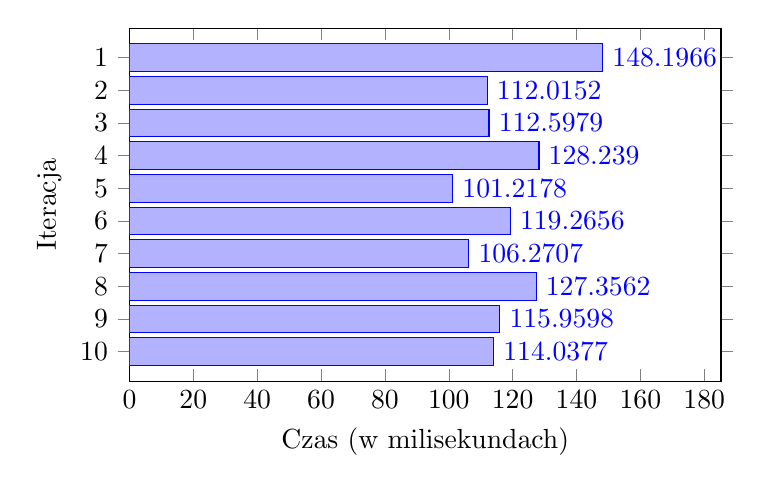
\begin{tikzpicture}
  
    \begin{axis} [
      xbar = .05cm,
      nodes near coords,
      nodes near coords style={
        /pgf/number format/precision=4,
      },
      xmin = 0,
      ytick = data,
      enlarge x limits = {value = .25, upper},
      symbolic y coords = {10,9,8,7,6,5,4,3,2,1},
      xlabel=Czas (w milisekundach),
      ylabel=Iteracja,
      width=0.75\textwidth,
      height=0.5\textwidth
    ]
    
      \addplot coordinates {(148.1966000199318,1) (112.0151999592781,2) (112.59790003299713,3) (128.2389999628067,4) (101.21780002117157,5) (119.26560002565384,6) (106.27069997787476,7) (127.3561999797821,8) (115.9598000049591,9) (114.03769999742508,10)};
      
    \end{axis}
  
  \end{tikzpicture}
  \caption{Wynik testów przykładu 3 [\ref{lst:wydajnosc-przyklad-p-3}]}
  \label{fig:wynik-przyklad-2}
\end{figure}
